\section{Language translation, semantic analysis}

Consider the source language $L_S$ generated by the grammar $G_S$, over the two-letter alphabet $\Sigma= {0,1}$:
\[G_S=\begin{cases}
    S \rightarrow 0Q|1R     \\
    Q \rightarrow 0S|1S|0|1 \\
    R \rightarrow 0S|1S|0|1 \\
\end{cases}\]
\begin{enumerate}
    \item Write a syntax scheme $G_{\tau}$ (or a translation grammar) for the translation $\tau$ over the source language $L_S$ defined as follows: 
        all couples of binary number must be translated into base four numbers. For example: 
        \[100111000 \rightarrow 2130\]
        The grammar generates strings of even length greater or equal than two. 
    \item Define the regular translation expression.
\end{enumerate}

\paragraph*{Solution}
\begin{enumerate}
    \item The translation grammar is defined as follows:
        \[G_{\tau}=\begin{cases}
            S \rightarrow \dfrac{0}{\varepsilon}Q|\dfrac{1}{\varepsilon}R     \\
            \\
            Q \rightarrow \dfrac{0}{0}S|\dfrac{1}{1}S|\dfrac{0}{0}|\dfrac{1}{1} \\
            \\
            R \rightarrow \dfrac{0}{2}S|\dfrac{1}{3}S|\dfrac{0}{2}|\dfrac{1}{3} \\
        \end{cases}\]
    \item The corresponding regular translation expression is given by:
        \[T_{\tau}=\left( \dfrac{00}{0}|\dfrac{01}{1}| \dfrac{10}{2}|\dfrac{11}{3}\right)^{+}\]
        The associated translation automaton is depicted below:
        \begin{figure}[H]
            \centering
            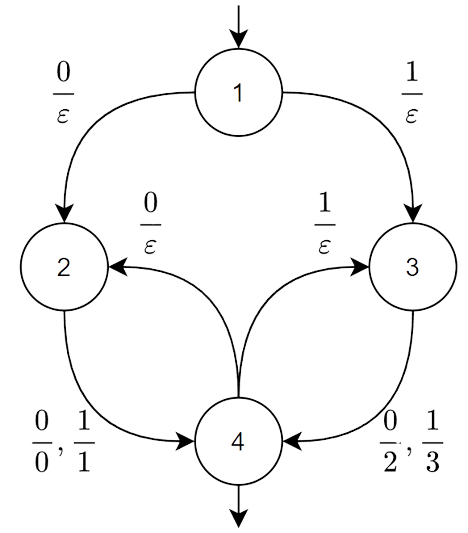
\includegraphics[width=0.4\linewidth]{images/gram.png}
        \end{figure} 
\end{enumerate}